\section{Introduction \label{sect:intro}}


\subsection{Scope \label{sect:scope}}

This document describes the scope and organizational concepts of the
{\bf LSST Data Management Science Verification} (DM SV) effort. 

\subsection{Background and Motivation for the Activity}

LSST Data Management subsystem is charged with delivering a fully functional
Data Management system capable of generating and serving to the community
the LSST data products as defined in the Science Requirements
Document (\SRD).  This overall mission has been flowed down to the
requirements and design of DM components and services, as described in the
DM branch of the project work breakdown structure (02C.02.*) and design
document referenced therein.

Assuming idealized conditions, once the project goals have been unambiguously
articulated and flowed down to (quantitative) definitions of requirements,
once those requirements have been validated to satisfy the mission need,
once design has been established to implement the requirements, and once the
plan has been established to build, integrate, and verify the components and
the system as a whole, it could be theoretically possible to build and
integrate the DM system by strictly adhering to the plan and and verifying
the as-built system against the original requirements only\footnote{This is,
roughly, the {\em waterfall model} of development.}.

Reality tends to settle from ideal conditions.  The
definition of the mission may not be sufficiently clear at the beginning of
the project (or may change).  The flow-down of requirements may contain
errors or not fully capture the metrics relevant to scientific success of
the mission.  The assumptions made while deriving requirements and designs
may not be born out by the real data.  Similarly, designs are possible that
satisfy formal requirements, but deliver unsatisfactory solutions that would
impede research with LSST (e.g., systems that are too complex).  Or designs
may make suboptimal trades (e.g., would require expenditure of significant
resources to perfect features that are by then recognized as unneeded).

A way to ensure that what's being built does not diverge from the ultimate goals
(as their understanding evolves and improves) is to periodically
exercise the integrated system as it's being built beyond piece-wise requirements
verification and, ultimately, with real data.  I.e., {\em
try to use it in ways we would expect it to be used by the stakeholders -- the
ultimate users of the system -- scientists}.  Such exercises close the
design-build-verify loop, and enable one measure the degree to which the
requirements, designs, and plans continue to satisfy stakeholder needs. 
Furthermore, they provide valuable feedback about modifications needed to
ensure the delivery of a scientifically capable system.

\subsection{Objectives }

The primary objective of this document is to define mechanisms by which we
will periodically verify that the DM system, as a whole, is on track to
being capable to acceptably support the science goals of commissioning and
operations: {\bf DM Science Verification}.

We define  {\bf DM Science Verification} as {\bf the assurance that the Data
Management system meets the needs of the scientific community and other
identified stakeholders}.  This follows the PMBOK 4th ed.  definition of
{\em validation}\footnote{It would have been more appropriate to name
this activity {\em Science Validation}; however, given the established use of
the term {\em Science Verification} on LSST and other large projects in the
U.S.  (e.g., DES, DESI, ALMA), we will continue to use
it.}\textsuperscript{,}\footnote{\url{https://en.wikipedia.org/wiki/Verification_and_validation}}

The solutions described below are a response to the responsibilities and
authorities delegated to the DM Project Scientist by R2A2 documents for the
LSST organization (LPM-???), and draw heavily on the Commissioning Plan, as
well as the Operations Plan.

\subsubsection{Science Verification}


To discuss DM Science Verification (SV), we coarsely break down and define
some aspects of Construction and Integration and Test procedures and how
they come together to ensure a functioning system is delivered.  While we
roughly define the roles and responsibilities for all parts of that process,
we do not dwell on the details of non-SV elements, namely {\em
verification}; these are beyond the scope of DM Project Science.  This
document focuses on Science Verification -- other elements are sketched out
as necessary to understand the scope and execution of SV.

\begin{figure}
\centering
\scalebox{0.6}{\hskip 0.0in 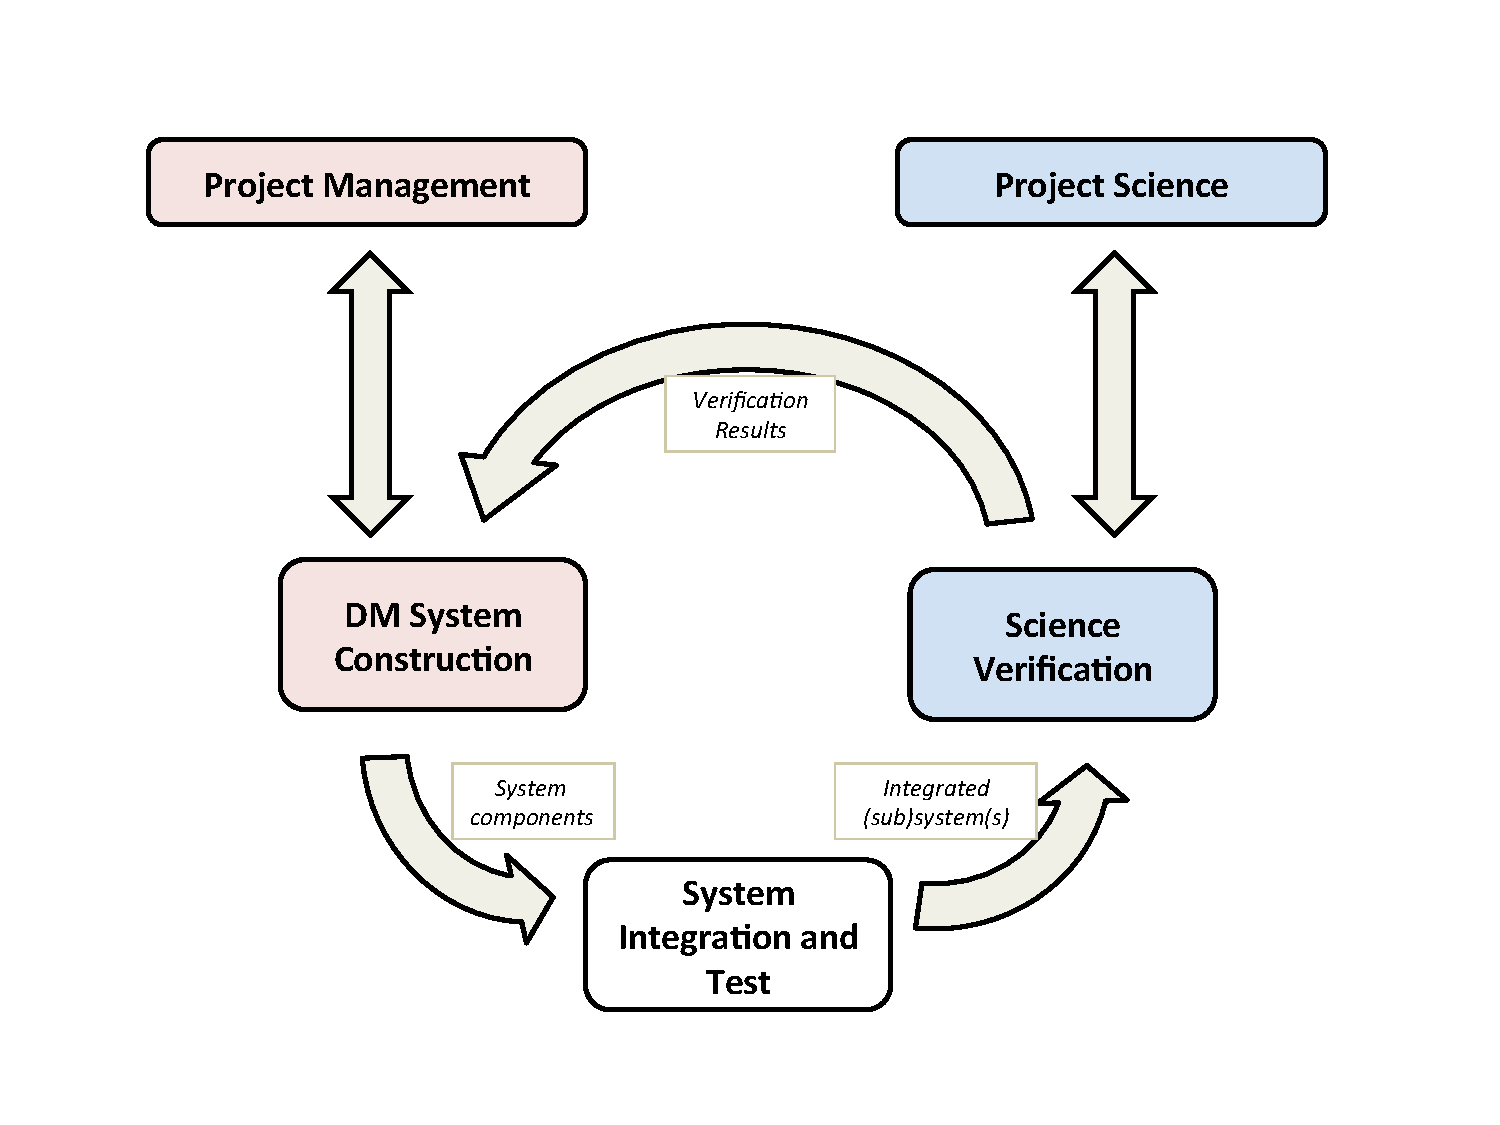
\includegraphics[trim={2cm 1cm 2cm 2cm},clip]{cycle.pdf}}
\caption{A graphical representation of the feedback loop from Science
Verification\label{fig:iterativeDevelopment}}
\end{figure}

% The DM System has been broken down into a number of work packages, each of
% which has been assigned to an institution to develop, deliver and (in some
% cases) operate. These deliverables need to be tested and integrated into the
% overall system, and then re-tested in the system as a whole. We identify
% three levels of quality assurance:

A schematic overview of the iterative process by which the LSST Data
Management system is built is shown in
Figure~\ref{fig:iterativeDevelopment}.  The cycle duration is roughly $\sim
6$ months.  Deliveries are represented by single-headed arrows connecting
the three boxes in the lower part of the diagram.  Each arrow presumes {\em
a battery of verification tests have been run} before the deliverables
were handed over to the next stage.

We (conceptually) divide the process into three stages:
%
\begin{itemize}

\item {\bf Component Construction}: The LSST WBS establishes that construction
partner institutions are responsible for delivering feature-complete,
tested, documented, work packages\footnote{It's typical for an entry in the
Work Package notebook to begin with ``{\em This WBS element includes
software programs, configuration files, unit tests, component integration
tests, and documentation that implement Foo...  }''; See
\href{http://ls.st/LPM-44)}{LPM-44} for details.}.  As such, upon hand-over
to I\&T, the {\em partner institutions are responsible for demonstrating
that their deliverables meet agreed upon requirements.}.  These tests,
developed by the partner institutions, will generally go beyond simple unit
tests; the expectation is that the delivered components will perform as expected
at their level of maturity when fed LSST-like data.  While they can
(and should) rely on an automated QC system to automate and execute these
tests, the responsibility for devising and writing them is with the partner
institution. Testing standards and procedures are described in a separate
document (LDM-503).

\item {\bf Integration and Test}: The operating institution (generally,
NCSA) is responsible for taking deliverables from the construction partners
and integrating them into increasingly capable and more integrated
prototypes of the DM System.  NCSA will, as a part of Integration and Test,
run a battery of quality assurance tests verifying against requirements the
functioning of the as-built system, and preventing unexpected regressions
relative to prior releases.  High level of integration of this and the
automated QC system mentioned above would be advantageous; optimally, the
I\&T of software components would be fully automated and continuous.

\item {\bf Science Verification}: The integrated prototypes of parts or the
whole DM system are delivered to the DM Project Science Group for Science
Verification.  The PSG devises and performs additional tests and data
challenges to exercise the integrated system and assess its quality relative to
expectations for the current phase of construction.  This assessment is
fed back to DM Project Science, Management, and Architecture, to inform
future development of the system.  The QA tests or procedures identified
as good metrics of system quality are also fed back to the I\&T team for
incorporation into the automated QC systems, to be run in the I\&T or
Component-level QA phases in the future, as appropriate.

\end{itemize}

An example of this process may be as follows:

\begin{itemize}

\item At the end of a 6-month cycle, Princeton University delivers to NCSA a
documented and internally tested set of DRP pipelines with a well defined
list of capabilities (for example, the Multifit implementation of the
moving point source model -- i.e., proper motions and parallax measurements).
The pipelines pass all unit and small-scale integration tests.

\item NCSA deploys and re-verifies the received pipelines in the I\&T
environment designed to closely mimic the production
environment\footnote{Nothing in this precludes a
DevOps-like design (e.g. see https://en.wikipedia.org/wiki/DevOps) of this
element of the system; it would be desirable if these kinds of deployments
were maximally automated.}. They verify that the pipeline integrates well
with the NCSA-delivered orchestration system and is capable of executing
medium-to-large scale processing. The pipelines pass integration tests.

\item With input from DM Project Management, the Science Verification team
designs, organizes, and coordinates a data challenge to stress the new
capabilities.  For example, a mini data release production using HSC data
could be devised to independently validate the proper motion measurements
beyond what is already included in the QC and I\&T tests.  The challenge is
executed by the proto-Operations team (e.g., the group at NCSA who will
execute the data release production in operations).  The analysis from the
end-user perspective is performed by the SV team.  The results and
conclusions derived from the data challenge are fed back to the DRP team, DM
Project Management, and DM Project Science; they may be used to assess the
overall quality of the product, pass a formal requirement, and/or inform
future construction decisions.  Any newly developed but broadly useful
tests are identified as such, and fed to the I\&T team for inclusion into the
battery of tests that are run on a regular basis.

\end{itemize}

%\subsection{Risk Factors}
%What can you identify as potential problems the contractor should take note of up front. Of course the contractor should perform their own risk assessment as well.
%
%
%\subsection{Applicable Documents \label{sect:ad}}
%When applicable documents change a change may be required in this document.
%\begin{tabbing}
%AUTH-NUM\= \kill 
%\citell{LL:AUTH-XXX} \>	DM Plan  \\
%\citell{LL:AUTH-XXX}\>	Other applicable doc \\
%\end{tabbing}
%
%\subsection{Reference Documents}
%
%\renewcommand{\refname}{}
%\bibliographystyle{gaia_aa}
%\bibliography{lsst,gaia_livelink_valid,gaia_drafts,gaia_refs,gaia_books,gaia_refs_ads}
%
%\subsection{Definitions, acronyms, and abbreviations \label{sect:acronyms}} 
%% include acronyms.tex generated by the acronyms.csh (GaiaTools)
%The following table has been generated from the on-line Gaia acronym list:
\newline\newline%decrement table counter so table sin doc start at 1.
\addtocounter{table}{-1}
\begin{longtable}{|l|p{0.8\textwidth}|}\hline 
\textbf{Acronym} & \textbf{Description}  \\\hline
API&Application Programming Interface \\\hline
CU&Coordination Unit (in DPAC) \\\hline
DM&Data Management (LSST) \\\hline
DPAC&Data Processing and Analysis Consortium \\\hline
DPACE&Data Processing and Analysis Consortium Executive \\\hline
ECSS&European Cooperation for Space Standardisation \\\hline
ESA&European Space Agency \\\hline
ESAC&European Space Astronomy Centre (VilSpa) \\\hline
ESF&European Science Foundation \\\hline
ESTEC&European Space research and TEchnology Centre (ESA) \\\hline
FOP&Flight Operation Procedure (Plan) \\\hline
GIS&(Astrometric) Global Iterative Solution \\\hline
IOA&Institute of Astronomy (Cambridge; also denoted IOA) \\\hline
LDAP&Lightweight Directory Access Protocol \\\hline
LSST&Large Synoptic Surrvey Telescope \\\hline
LTD&LSST the Docs \\\hline
LaTeX&(Leslie) Lamport TeX (document markup language and document preparation system) \\\hline
MDB&Main Database \\\hline
MOC&Mission Operations Centre \\\hline
NASA&National Aeronautics and Space Administration (USA) \\\hline
PR&Progress Report \\\hline
QA&Quality Assurance \\\hline
SDSS&Sloan Digital Sky Survey \\\hline
SOC&Science Operations Centre \\\hline
SVN&SubVersioN \\\hline
TOC&Table of Contents \\\hline
USA&United States of America \\\hline
WP&Work Package \\\hline
XMM&X-ray Multi-mirror Mission (ESA; officially known as XMM-Newton) \\\hline
\end{longtable} 


\section{Organization, and Schedule }

\subsection{Organization}

\begin{figure}
\centering
\scalebox{0.5}{\hskip 0.0in 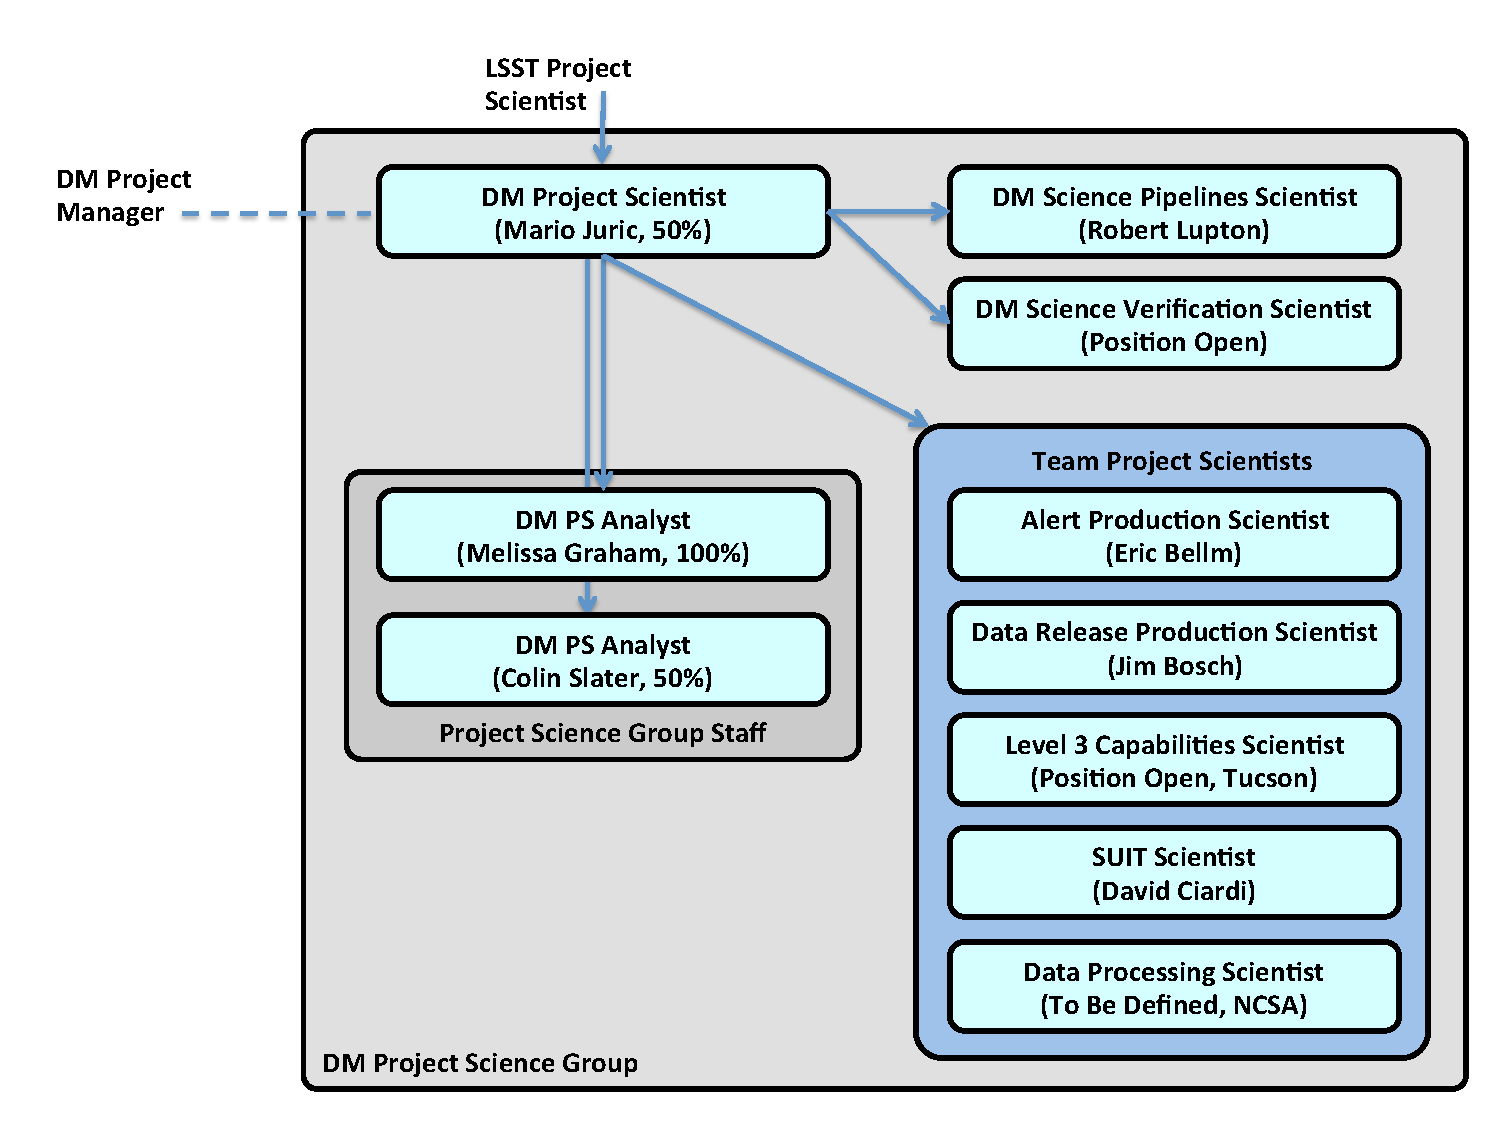
\includegraphics[trim={0cm 0cm 0cm 0cm},clip,page=1]{dm-psg.pdf}}
\caption{Organogram of the Data Management Project Science Group. DM Science
Verification is the responsibility of the Project Science Group, coordinated
by the Science Verification Scientist.\label{fig:DMpsg}}
\end{figure}

The DM Project Scientist is accountable to the LSST Project Scientist for
the success of DM Science Verification activities.  They delegate the
responsibility for the coordination of Science Verification activities to
the DM Science Verification Scientist\footnote{This position has previously
been called the ``End-to-end Scientist''; the change has been made to
harmonize the terminology with the Commissioning Plan where analogous
activities take place using real LSST data.}.  SV activities draw on
resources of the DM Project Science Group\footnote{Our first choice would be
to call this group the {\rm DM Project Science Team}, consistent with the
terminology elsewhere in DM, but because of potential confusion with the
project-level {\em Project Science Team} we choose the title ``Group''}
(Figure~\ref{fig:DMpsg}), but may also tap into the broader construction
team if needed (and as jointly agreed upon with the DM Project Manager), as well
as contributors from the LSST Science Collaborations.  Decisions on
strategic goals of SV exercises are made in close consultation and
coordination with the DM Project Manager; for example, it would be expected
that the SV team would be downstream of dress rehearsal activities,
receiving any generated data.

\begin{figure}
\centering
\scalebox{0.5}{\hskip 0.0in \includegraphics[trim={2.4cm 3cm 2.4cm 3cm},clip,page=2]{dm-psg.pdf}}
\caption{Organogram of the Data Management Science Verification Group. 
The group is chaired and coordinated by the DM Science Verification Scientist,
with the DM Science Pipelines Scientist and Team Project Scientists making up
the permanent membership. Depending on the SV activities being executed at any
given time, the group may draw on additional temporary members from DM PSG Staff,
the broader DM Construction staff, as well as external scientists (e.g.,
Science Collaboration members committed to assisting SV goals). SV membership
is reassessed on a cycle by cycle basis, with estimates incorporated in the
long-term plan.
\label{fig:DMsvg}}
\end{figure}

Participants in SV activities make up the Science Verification Team. 
The team is lead by the DM SV Scientist. The SV Scientist, the DM Science
Pipelines Scientist, and all Team Project Scientists are ex-officio members
of the SV Team. DM Project Scientist and Managers are not formal members,
but monitor the work of the group. Additional members may added as
needed, depending on SV activities being considered and based on the
recommendation of the DM SV Scientist and resource constraints. This is
illustrated in Figure~\ref{fig:DMsvg}.

\subsubsection{Stakeholders}

{\bf DM Project Scientist} commissions and accepts the results of SV
activities.  The results (reports) are used to inform actions of the DM
Project Science Group (as Product Owners) while articulating DM development
priorities and maintaining the overall DM system vision.

The DM PS informs the {\bf DM Project Management} of SV results and recommendations. 
The DM Project Manager can use these to assess current development
status, measure performance, make development adjustments, and generally
enhance their awareness of the actual state of the system relative to
the plan.

The DM PS reports the results and recommendations to the {\bf LSST Project
Scientist}. The LSST PS uses the reports to maintain awareness of the
status and progress of the LSST Data Management subsystem, as well as direct
the activities of the DM Project Scientist.

\subsubsection{Transition to Updated Organization}

At the moment, the SQuaRE scientist holds responsibilities closest to those
of the DM SV Scientist role.  Following the departure of David Nidever, this
position is currently open, with Michael Wood-Vasey (U.  Pitt) serving in an
interim role at 25\%.

Following the adoption of this document, the SQuaRE scientist
responsibilities will be reassigned to two new positions:
%
\begin{itemize}
\item {\bf Level 3 Scientist}: with the responsibility to serve as the Product Owner
for the Level 3 services aspects of the LSST Science Platform (and possibly
other areas), and
\item {\bf SV Scientist}: with the responsibility to lead and coordinate the work
of the DM Science Verification group, as described in this document.
\end{itemize}
%
Some responsibilities presently delegated to the SQuaRE scientist, such as
collection and curation of science verification datasets, or the definitions
of code modules to measure the very high-level key performance metrics
(KPMs), will revert to the Project Science Group (and be specifically
delegated to designated staff).  For example, KPMs measuring the quality
of DRP-derived products (e.g., TEx measures of PSF correlations) are most
naturaly owned by the DRP Scientist as the Product Owner in that area. 
This has already partly taken place.

These activities are integral to the SV aspect of DM Project Science role,
but will obviously greatly assist CI and I\&T activities.  The collection
and curation of datasets and execution of metrics will be done in close
collaboration with the DM Construction team.  I.e., it should utilize the
same tooling, databases, etc.  that the Construction team provide and use
for I\&T themselves.  The systems on which SV will be performed, and the
(e.g., visualization) widgets used, will be developed by the DM
Construction team.

\subsubsection{Evolution into Commissioning}

[[ TO BE WRITTEN (basically, the SV team (and all of its tools and processes) continue
into commissioning -- the nature of the work is qualitatively the same). 
{\bf We're effectivelly building the Commissioning SV team here, that Chuck
\& Zeljko smoothly inherit in $\sim$2020}.  Chuck will be at UW next week to make sure
this responds to the needs of the Commissioning Plan. ]]

\subsubsection{Evolution into Operations}

[[ TO BE WRITTEN (some in the SV team may join the Science Ops team, making it
possible to smoothly transfer experience and expertize to the new LSST
Center). ]]

\subsection{Schedule}

DM SV activities are planned and prepared in a rolling wave fashion in
parallel with development activities (on a 6-month cycle, or perhaps a
year).  The SV activities will typically be designed so as to exercise the
capabilities of the system expected to be delivered at the end of a given
development cycle.  There shall exist a long-term roadmap of SV activities,
linked to product delivery milestones in the DM's Construction Plan.  The
definition and design of SV activities will be performed in close
consultation with the DM Project Manager.

By their nature, SV activities will typically lag behind
deliveries of the (sub)system being verified -- ideally, they will commence
immediately upon delivery. Preparatory SV activities (e.g., identification and
acquisition of suitable datasets, identification of potential Science
Collaboration resources to include on the activity, or development of
activity-specific analysis codes) will commence as early as feasible. DM SV
Scientist will coordinate the execution of all SV activities.

SV activities should aim to take no longer than two months to conclude, to
enable rapid actionable feedback to DM Management and DM Project Science.

\section{Work to be performed} \label{sect:wps}

The Project Science Group will design and execute SV activities to assure
that the Data Management system meets the needs of the scientific community
and other identified stakeholders as described in the previous section.

%\subsection{{\bf WP-01:} Some work we want done \label{wp1}}
%Description of the work to be done
%
%Can use requirements labels to tag paragraphs for traceability..
%
%
%  \newreqtype{WP-1}
% \req[]{1.0}{FUNC}{HIGH}{AUTO}{Draft}
%         {      \label{req:wp1:sometask}
%The important piece of work will be done in such and such a manner. \ldots
% }


\subsection{Project Management, Reporting and Meetings}

\subsection{Management}

The DM Project Scientist will be accountable for the execution of Science
Verification activities. They delegate their responsibility in the area to
the {\bf DM SV Scientist}.

The DM SV Scientist will be responsible for proposing, planning, and
executing all SV activities. The SV Scientist will be the CAM for the
account out of which SV activities are funded.

\subsubsection{DM SV Scientist: R2A2 Breakdown}

[[ TO BE WRITTEN ]]

\subsection{Reporting}

DM SV Scientist will regularly report on the status of SV activities to the
DM Project Scientist.

The DM Project Scientist will regularly inform the DM Project Manager and
the LSST Project Scientist of the status of ongoing SV activities.

All SV activities will conclude with a written report, accepted by the DM
Project Scientist. The SV Scientist is responsible for the writing and
submission of the report.

\subsection{Meetings and Travel}

The SV Team will meet via video as often as needed to ensure the success of
SV activities.

The SV Team members will travel for in-person meetings as needed to ensure
the success of SV activities, within the constraint of the available travel
budget.

\section{Deliverables}

Key deliverables of Science Verification activities are:
\begin{itemize}

\item Reports on the measured capability of the Data Management System to
satisfy stakeholder needs.  The assessments shall take into account the
expected maturity of the system being tested.

\item Recommendations for improvements and changes, both in the quality of
as-constructed systems (i.e., what needs to be built differently or better,
to make it more consistent with the system vision) as well as the overall
system vision (i.e., where the vision needs to be changed to better address
stakeholder needs).

\item Measurements of performance metrics that do not lend themselves to
easy automation (e.g., science activities requiring human involvement, like
visual classification, or UX tests).  Development of new performance
metrics, including potential deliveries of code to the DM Construction and
I\&T teams for inclusion in automated pipelines.

\item Other deliverables as charged when chartering a particular SV exercise.

\end{itemize}

\section{Deliveries to the SV Team}

The DM I\&T team shall deliver to the DM SV team the system or systems being
tested, that have already passed formal requirements verification to the
degree agreed upon when the SV activity was chartered\footnote{We leave this
caveat to make room for formal activities which themselves may be verified
by the SV activity.}.

The DM Construction team shall deliver to the DM SV team the quality
assessment tools and widgets (e.g. JupyterHub system with access to
prototype data products, or visualization widgets used to explore LSST
data) needed for successful execution of the SV effort.
